\section{Propriedades}
As propriedades do material necessários para a simulação são a condutividade
térmica, o calor específico, a densidade, a permeabilidade e a água quimicamente
ligada, conforme apresentadas na Figura \ref{fig:properties}.

 \begin{figure}[ht]
\centering
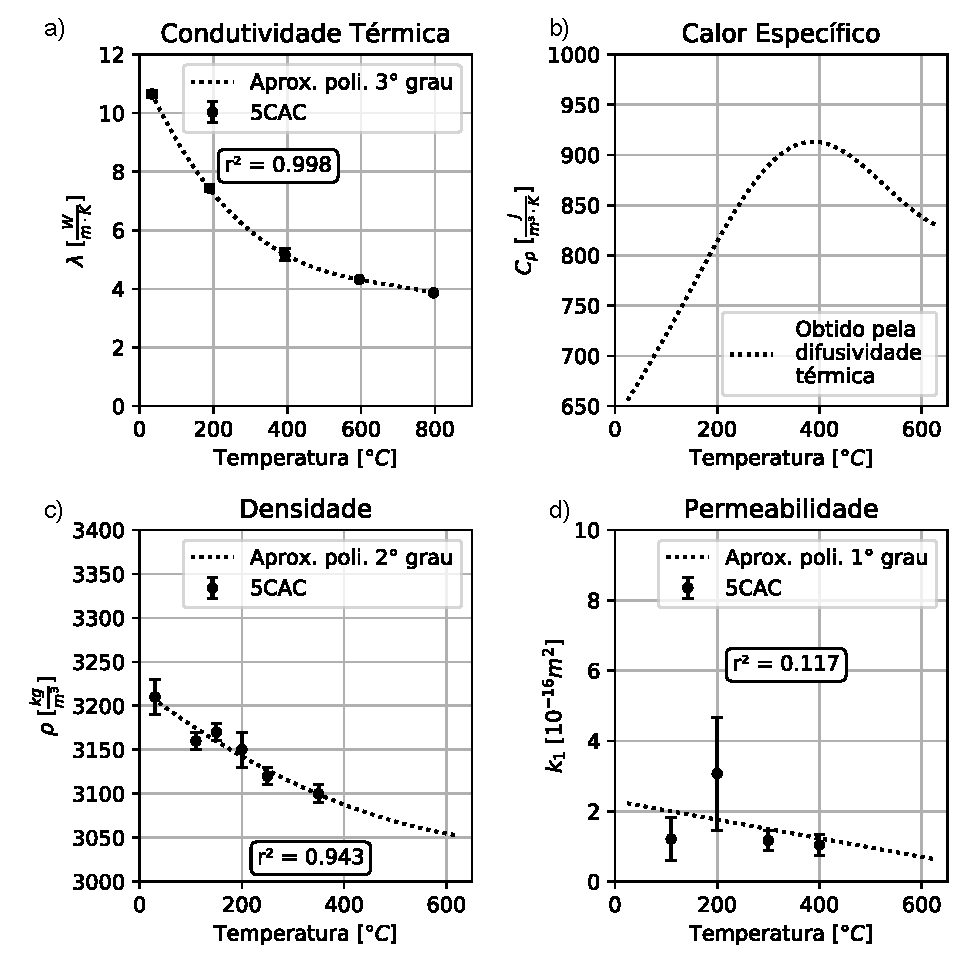
\includegraphics[width=14cm]{./figures/properties.pdf}
\caption{Caracterização da composição de concreto refratário utilizado no
  presente estudo, (a) condutividade térmica, (b) calor espicífico, (c)
  densidade e permeabilidade (d).  \label{fig:properties}}
\end{figure}

A condutividade térmica decaí conforme a temperatura aumenta. Tal comportamento
pode ser aproximado por um polinômio de terceiro grau. Este comportamento
justifica-se pelo aumento da frequência de oscilações dos átomos, o que diminui
o caminho livre médio dos fónons que são os principais transportadores de
energia térmica até aproximadamente 800$^\degree$C quando o transporte por
radiação começa a predominar \cite{pelissari2017}. A densidade é reduzida devido
a liberação da água físicamente adsorvida, bem como a água quimicamente ligada.
Outro efeito provável é a conversão de fases menos densas do cimento aluminoso
hidratado em fases de maior densidade, o que amplia a porosidade do material. O
calor específico foi calculado a partir da medida de difusividade térmica,
$\alpha = \frac{\lambda}{\rho \ C_p}$, e portanto não é apresentado o desvio
associado. Por fim, a permeabilidade do material apresenta um desvio padrão
muito elevado, e isto reflete no baixo valor de $r^2$ (aqui uma possível solução
seria aumntar o grau do polinômio, porém, seria o equivalente a realizar um {\it
  overfitting} uma vez que estaríamos inserindo no modelo um comportamento que
pode ser apenas o produto do erro da medida \cite{raschka2017}). 

 \begin{figure}[ht]
\centering
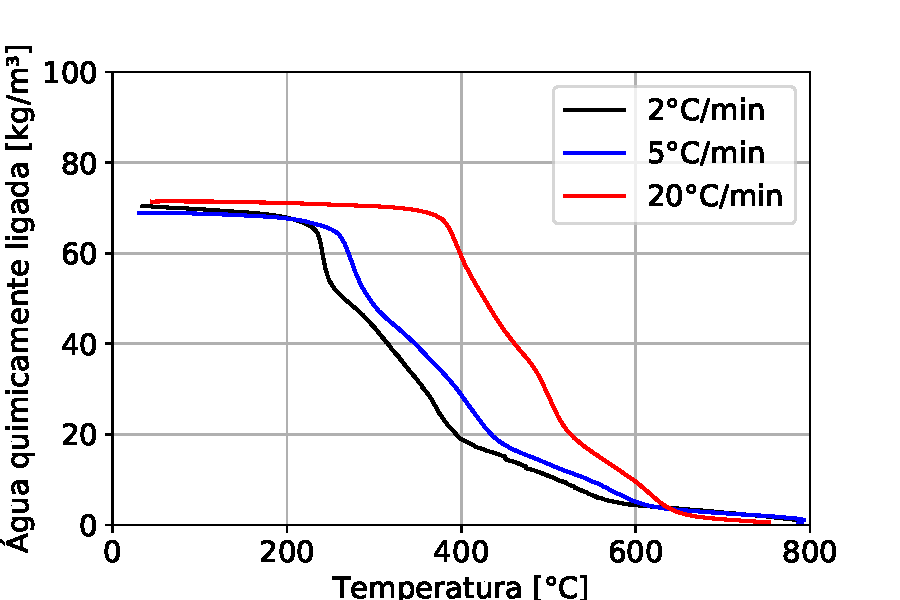
\includegraphics[width=14cm]{./figures/w_d.pdf}
\caption{Água quimicamente ligada por $m^3$ de concreto.  \label{fig:prop_wd}}
\end{figure}

Na Figura \ref{fig:prop_wd} a curva de liberação de água químicamente ligada é
apresentada. Sua medição é realizada a partir do ensaio de TGA realizado em
amostras previamente secas à 110$^\degree$C por 24 horas. Tal abordagem deve ser
considerada cuidadosamnte uma vez que sua precisão precisa ser investigada mais
a fundo. Uma possível problemática envolvida nessa maneira de medir a água de
desidratação é a formação de fases específicas durante a secagem a
110$^\degree$C, que não estariam presentes em uma secagem do material apenas
curado.



Uma útlima propriedade fundamental para o modelo são as curvas de sorção
isotérmicas que representam a quantidade de água evaporável (líquida e
adsorvida) no material. Tais medidas são complexas e segundo Baroghen-Bouny REF,
para se ter medidas confiáveis o método de medida deve ser o método estacionário
com soluções salinas para controle de umidade relativa. Tais ensaios podem
demorar meses até se atingir uma massa de água adsorvida constante no material.
Além da restrição de tempo, há uma notável hesterese quando comparado os
comportamentos de sorção e adsorção que devem ser levados em conta na medida.
Como alternativa, há o uso do método dinâmico de sorção de vapor, utilizado por
Fey et al \cite{Fey2016b}, cuja validade das medidas é limitado até 75\% de umidade
relativa.

Assim a metodologia adotada no presente trabalho foi utilizar as próprias curvas
adotadas por Ba\v{z}ant, porém, corringido os valores de água de saturação a
temperatura ambiente por metro cúbico de concreto, $w_0=\psi_0=0.0393 \ \rho_l$
e a quantidade de cimento por metro cúbico de concreto, $w_c= 0.05 \ \rho_c $.

\section{Ensaios para \textit{Benchmarking}}
Teste 2

\section{\textit{Benchmark} do modelo}
Teste 3 



%%% Local Variables:
%%% mode: latex
%%% TeX-master: "TCC-Secagem"
%%% End:
